\section{Obiettivi e valori}

\medskip
\noindent\textbf{Obiettivi}

L'azienda persegue obiettivi strategici chiari e complementari: da un lato il rafforzamento e l'aggiornamento continuo delle competenze interne attraverso progetti di ricerca e sviluppo e percorsi formativi
strutturati; dall'altro l'orientamento al cliente mediante offerte modulari e scalabili, pensate per ampliare la base clienti includendo sia piccole e medie imprese sia grandi committenti e,
quando opportuno, pubbliche amministrazioni. 
La strategia tecnologica è focalizzata sull'innovazione applicata: lo sviluppo di \emph{proof of concept} e soluzioni progettate per il \emph{cloud} favorisce
scalabilità e tempi di immissione sul mercato ridotti. 
Infine, la sostenibilità operativa e l'efficienza dei processi sono obiettivi trasversali, perseguiti con l'ottimizzazione dell'uso
delle risorse per contenere i costi e ridurre l'impatto ambientale dei servizi erogati.

\begin{figure}[htbp]
    \centering
    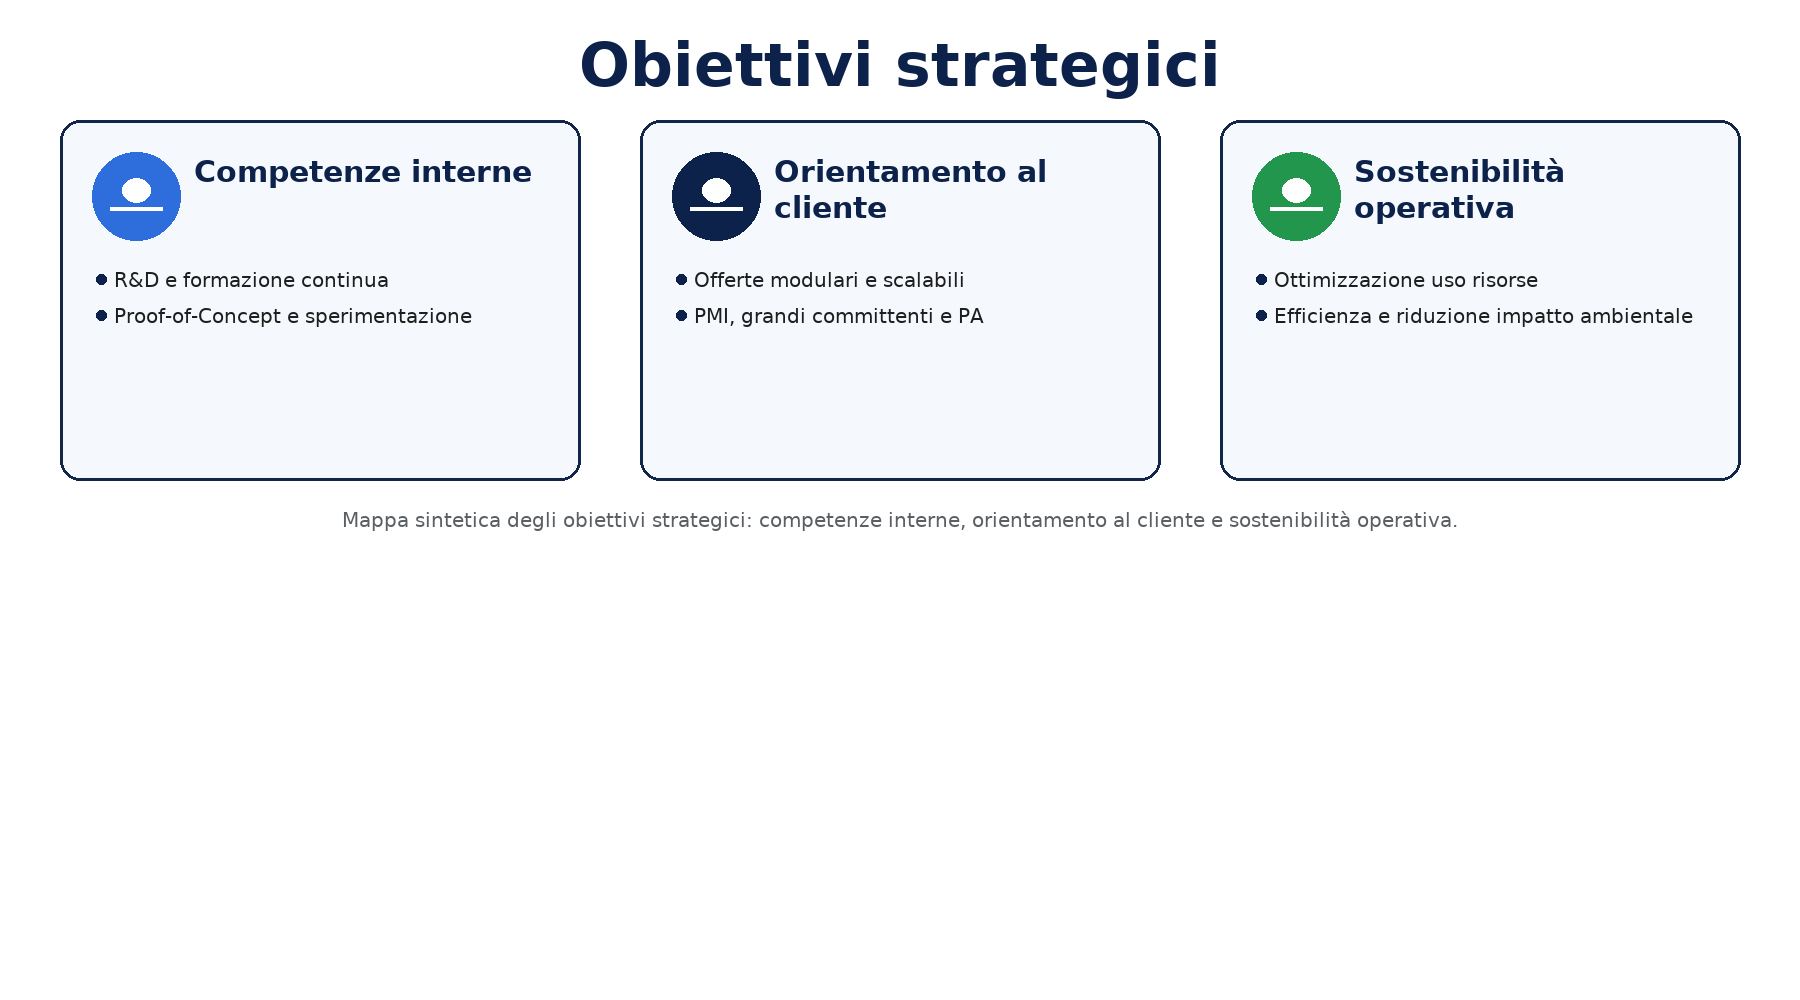
\includegraphics[width=0.8\textwidth]{images/azienda/obiettivi_strategici}
    \caption{Mappa sintetica degli obiettivi strategici dell’azienda: competenze interne, orientamento al cliente e sostenibilità operativa.}
    \label{fig:obiettivi}
  \end{figure}

\medskip
\noindent\textbf{Valori promossi}

I valori aziendali sostengono e rendono praticabili gli obiettivi strategici: la trasparenza e la responsabilità sono poste come fondamento dei
rapporti interni e delle relazioni con i clienti, favorendo chiarezza nelle comunicazioni e responsabilità nelle decisioni. La collaborazione e
la condivisione delle conoscenze sono considerate essenziali per evitare \emph{silos} informativi e per accelerare la diffusione delle competenze;
ciò si traduce in pratiche quotidiane come revisioni tecniche, sessioni di formazione interna e condivisione di documentazione.
L'etica professionale e la \emph{compliance} normativa rivestono un ruolo centrale soprattutto nei progetti con vincoli regolamentari:
si presta particolare attenzione alla protezione dei dati personali, alla sicurezza e alle procedure richieste per operare in settori regolamentati, garantendo così affidabilità e conformità.


\begin{figure}[htbp]
    \centering
    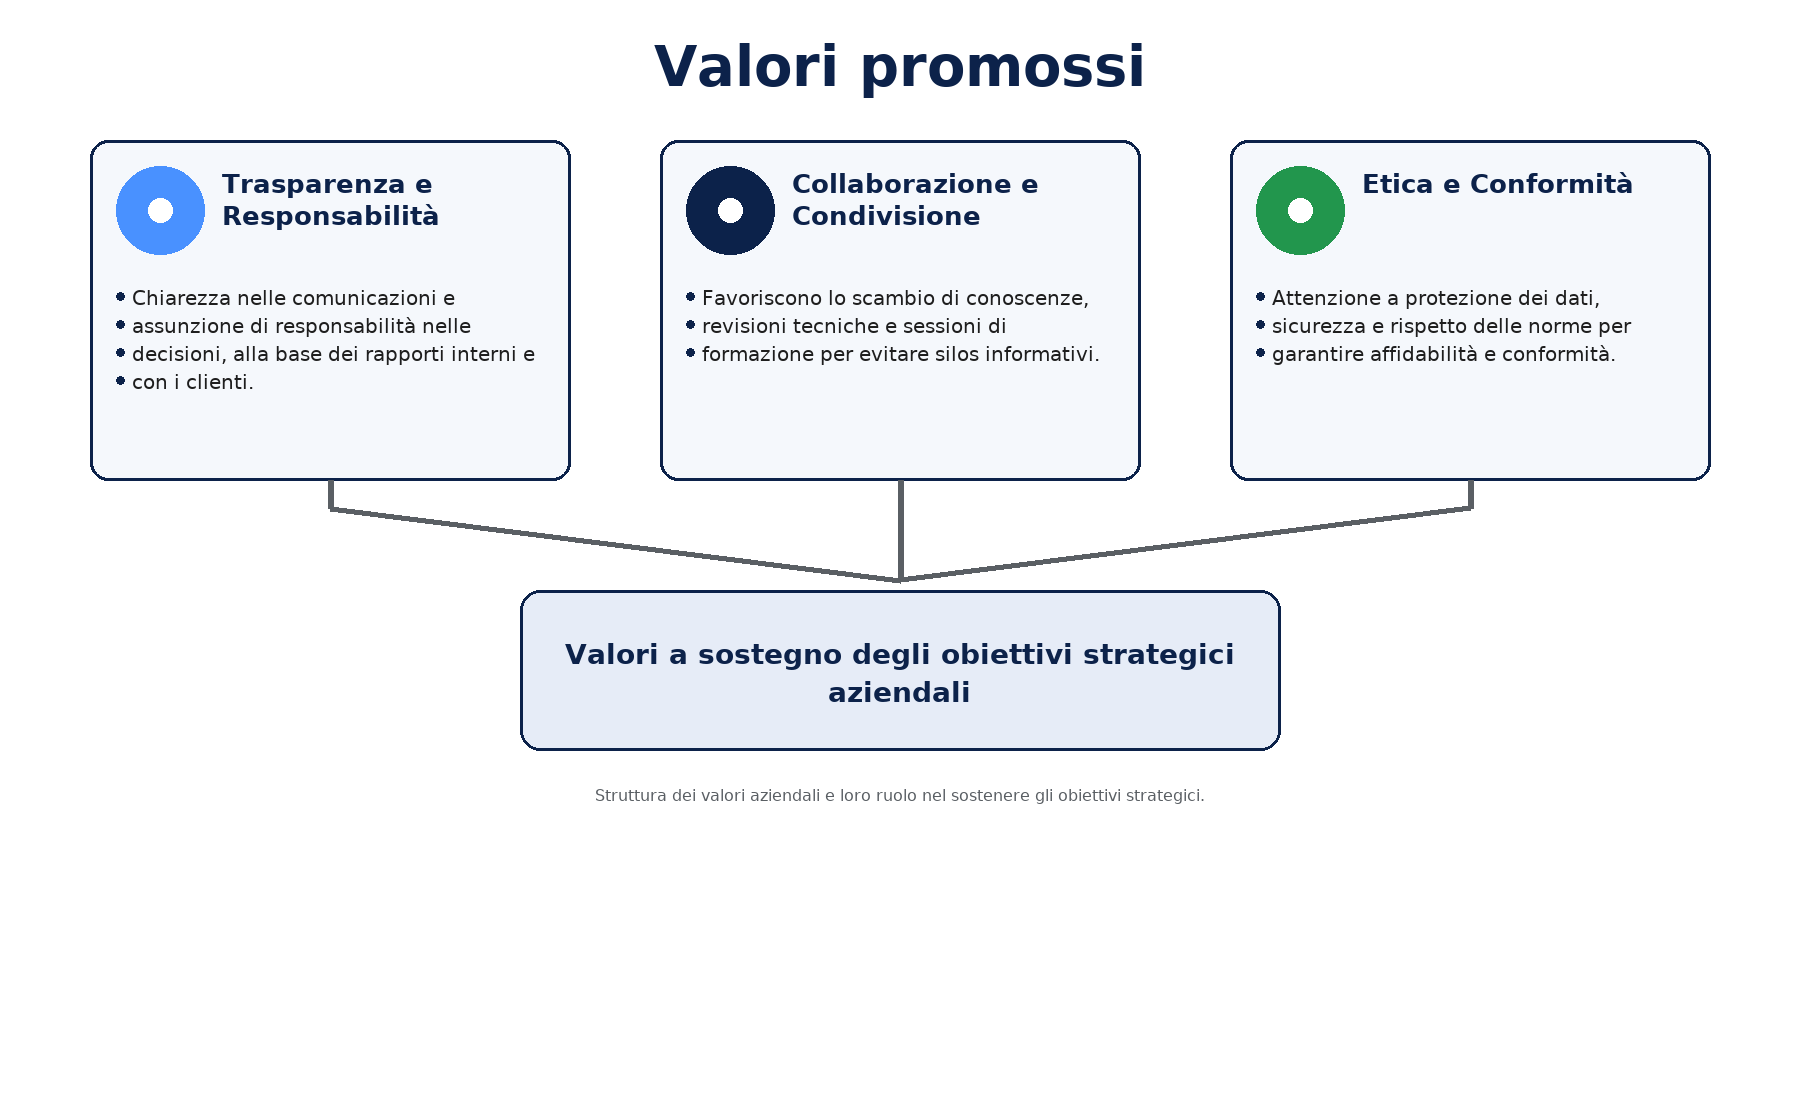
\includegraphics[width=0.8\textwidth]{images/azienda/valori_promossi}
    \caption{Struttura dei valori aziendali e loro ruolo nel sostenere gli obiettivi strategici.}
    \label{fig:valori}
\end{figure}

%diagramma a tre livelli o “piramide dei valori” Livello 1 (base): Etica e compliance Livello 2: Collaborazione e condivisione Livello 3 (apice): Trasparenza e responsabilità

\medskip
\noindent\textbf{Collegamento tra obiettivi, valori e contesto operativo}

Le scelte tecnologiche e i processi interni sono allineati agli obiettivi e ai valori dichiarati: l'adozione di architetture basate su microservizi e \emph{container},
\emph{pipeline} \emph{CI/CD} e sistemi di monitoraggio centralizzato facilita il rilascio rapido e controllato di nuove funzionalità, mantenendo al contempo la qualità e la stabilità di sistema.
L'adozione di pratiche \emph{Agili} e la gestione delle richieste tramite sistemi di \emph{ticketing} consentono di prioritizzare il lavoro, tracciare il debito tecnico e coordinare interventi
di manutenzione e \emph{delivery}. Questa combinazione di agilità operativa e rigore procedurale permette di conciliare la necessità di innovare rapidamente con l'esigenza di rispettare
vincoli normativi e contrattuali imposti da una \emph{clientela} eterogenea. Inoltre, gli investimenti in \emph{PoC} e le collaborazioni esterne con partner tecnologici e realtà accademiche
rafforzano la cultura dell'apprendimento e della sperimentazione, offrendo percorsi strutturati per valutare nuove idee prima della loro integrazione in produzione.

\medskip
\noindent\textbf{Impatto sulle relazioni interne e sul mio inserimento}

Gli obiettivi e i valori aziendali hanno influenzato direttamente il mio inserimento operativo: mi è stata concessa ampia autonomia nello svolgimento delle attività,
pur mantenendo un contatto costante con il \emph{team} attraverso momenti di sincronizzazione e confronto. L'\emph{onboarding} ha previsto l'assegnazione di una postazione in ufficio e
l'integrazione nei canali di comunicazione del \emph{team} (ad esempio \emph{Slack}), strumenti che hanno facilitato l'accesso alle informazioni, la partecipazione a \emph{stand-up} e la
visibilità sul \emph{backlog} di progetto. Questo ambiente ha favorito sia il mio coinvolgimento in attività di sviluppo pratico sia l'esposizione a fasi di ricerca e \emph{PoC},
permettendomi di apprendere rapidamente le pratiche aziendali—dal flusso di rilascio alle revisioni tecniche—e di ricevere \emph{feedback} strutturati volti al miglioramento continuo.